\section{Testomgeving}
\label{sec:testomgeving}
In de voorgaande secties werd beschreven hoe de implementatie van GeoSPARQL gemaakt is. Nu er een werkende implementatie is, is het mogelijk om over te gaan naar de volgende stap. Hier zijn drie doelen bij, namelijk:
\begin{enumerate}
    \item Visualiseren van het geheel, met makkelijk aanpasbare queries.
    \item Omgeving voor het geven van demonstraties van de implementatie.
    \item Omgeving voor het uitvoeren van tests, voor het aftoetsen van de hypothesen.
\end{enumerate}

Om dit te bereiken is gebruik gemaakt van de ``jQuery Widget'' van Comunica. Deze geeft een grafische \textit{user interface}, die toestaat om te queryen over één of meerdere bronnen. Hierbij is het mogelijk om de bronnen zelf in te geven. Daarnaast is het ook mogelijk om de query zelf in te geven. Deze geeft een overzicht van het resultaat terug en geeft een ``execution log'' terug, zodat gecontroleerd kan worden welke stappen doorlopen werden voor het bekomen van het resultaat. Het geheel hiervan is zichtbaar in \figureref{fig:testomgeving}.

\begin{figure}
    \centering
    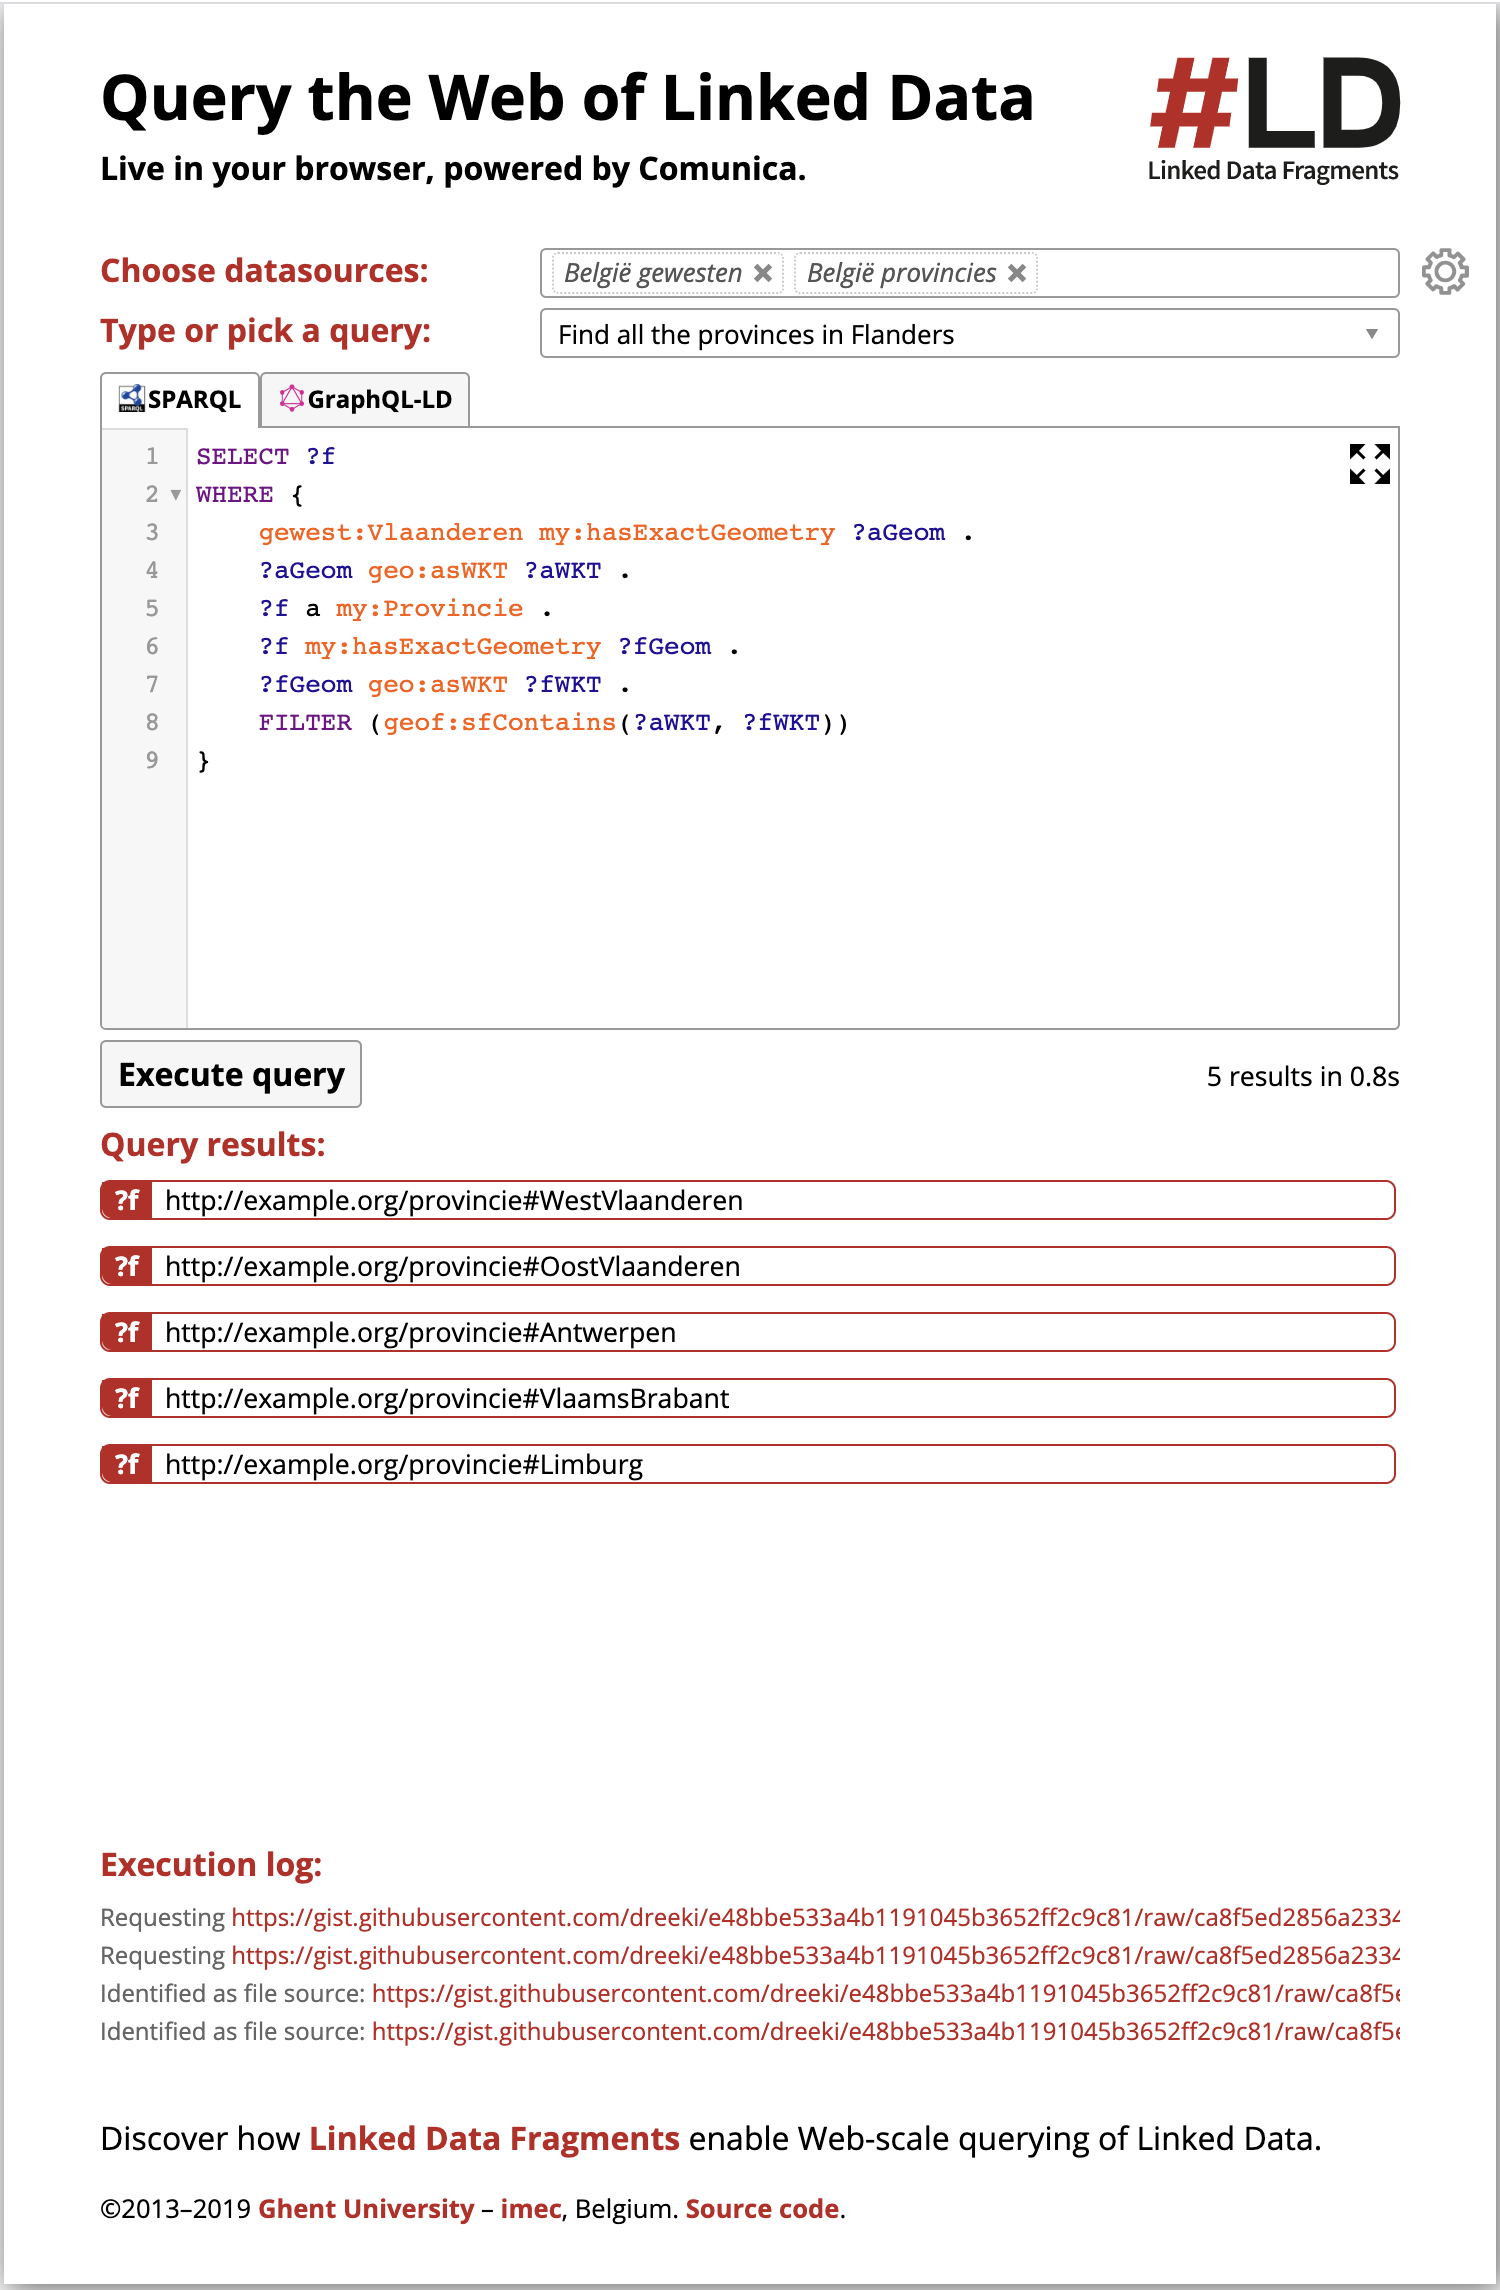
\includegraphics[width=0.8\linewidth]{images/testomgeving.png}
    \caption{Screenshot van online geplaatste testomgeving.}
    \label{fig:testomgeving}
\end{figure}

Hiermee is het eerste doel onmiddelijk bereikt. Dankzij het uitzicht dat zeer gelijkaardig is aan andere gekende \textit{query engines}, is dit zeer geschikt voor het geven van demonstraties. Ten slotte, zoals eerder vermeld, is het mogelijk om zowel de bronnen in te geven als de volgorde van uitvoering te bekijken. Hierdoor is het uitermate geschikt voor het uitvoeren van tests en voor het aftoetsen van de hypothesen.